\documentclass[11pt, letterpaper]{article}
\usepackage{color}
\usepackage[linktoc=all]{hyperref}

\usepackage[bindingoffset=0.2in,left=1in,right=1in,top=0.5in,bottom=1in,footskip=.25in]{geometry}
\usepackage{enumitem}
\usepackage{graphicx}
\usepackage{subcaption}
\usepackage{mwe}
\usepackage{parskip}
\usepackage{indentfirst}
\usepackage{textcomp}
\usepackage[formats]{listings}
\usepackage{xcolor}
\usepackage{geometry}
\usepackage{float} % keep figure fixed location with [H]
\definecolor{listinggray}{gray}{0.9}
\definecolor{lbcolor}{rgb}{0.9,0.9,0.9}
\definecolor{Darkgreen}{RGB}{11,100,35}

\geometry{
	body={7.0in, 9.8in},
	left=0.75in,
	top=0.6in
}

\hypersetup{
	colorlinks,
	citecolor=black,
	filecolor=black,
	linkcolor=black,
	urlcolor=black
}

\lstdefineformat{Java}{%
\{=\newline\string\newline\indent,%
\}=[;]\newline\noindent\string\newline,%
\};=\newline\noindent\string\newline,%
;=[\ ]\string\space}

\lstset{
	backgroundcolor=\color{lbcolor},
	upquote=true,
	language=Java,
	captionpos=b,
	tabsize = 4, %% Sets tab space width.
	basicstyle = \small \ttfamily , %% Sets listing font and size.
	breaklines = true, %% Enables line breaking.
	numberstyle = \tiny,
	frame=single,
	numbersep=5pt,
	prebreak = \raisebox{0ex}[0ex][0ex]{\ensuremath{\hookleftarrow}},
	basicstyle=\footnotesize,
	identifierstyle=\ttfamily,
	basicstyle=\scriptsize,
	showstringspaces = false, %% Prevents space marking in strings, string is defined as the text that is generally printed directly to the console.
	numbers = left, %% Displays line numbers on the left.
	commentstyle = \color{Darkgreen}, %% Sets comment color.
	keywordstyle = \color{blue}, %% Sets  keyword color.
	stringstyle = \color{red}, %% Sets  string color.
	rulecolor = \color{black}, %% Sets frame color to avoid being affected by text color.
}

\setlength{\parindent}{15pt}
%opening
\title{\textbf{Final Report}}
\author{En li, Yangde Li, Yangxiao Wang}



\begin{document}
	
	\maketitle
	
	\tableofcontents
	\pagebreak
	
	\section{Application Overview}
	For project 5, we implemented the Ant Colony Optimization of Traveling Salesman problem. The Ant Colony Optimization imitates real ant colonies. When ants look for food on the ground. a group of ants will each explore different route. If they find food, on their way back, they release Pheromones to mark the route for later searchers. When more ants explore a good routes, Pheromones on the route becomes more intense. Routes with heavier Pheromones will take precedence over routes with lighter Pheromones in the future. To encourage ants to explore different route and avoid local optima, we introduce a evaporation rate to adjust Pheromones at each iteration. We use these information to calculate a probability for each ant to move from city i to city j using the following formula: \par
	\begin{figure}[!htb]
		\centering
		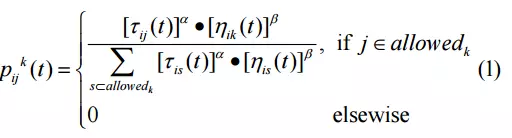
\includegraphics[width=0.6\textwidth]{sum}
		\caption{Probability formula}
	\end{figure}
	There are three ways to update Pheromones in Ant Colony Optimization:  Ant Cycle, Ant Density and Ant Quantity. We used the Ant Cycle model as it is more straight forward. In Ant Cycle model, the change in Pheromone is calculated by diving the current Pheromone by the total distance of the route calculated for current iteration if the ant passed through a given city pair, if the ant did not pass through the city pair, there is no change in Pheromone for this iteration.
	
	
	\section {Parallelization techniques}
	
	\subsection{MpiJava}
		In this implementation with MpiJava, we mainly focus on two types of parallelism techniques: \textbf{Task} and \textbf{Data} decomposition. For the task decomposition, we split the ants to different computing nodes, thus to accelerate whole computing speed. In every optimization loop, the worker nodes send back the delta pheromone generated by the ants in this iteration to master, then master updates the whole pheromone matrix and scatter it to all workers. Another parallel technique is to make every worker run a complete ACO process and update the pheromone matrix using mean value, this is a way to increase the ants searching space and increase the possibility of finding the best path.
	
	\begin{figure}[H]
		\centering
		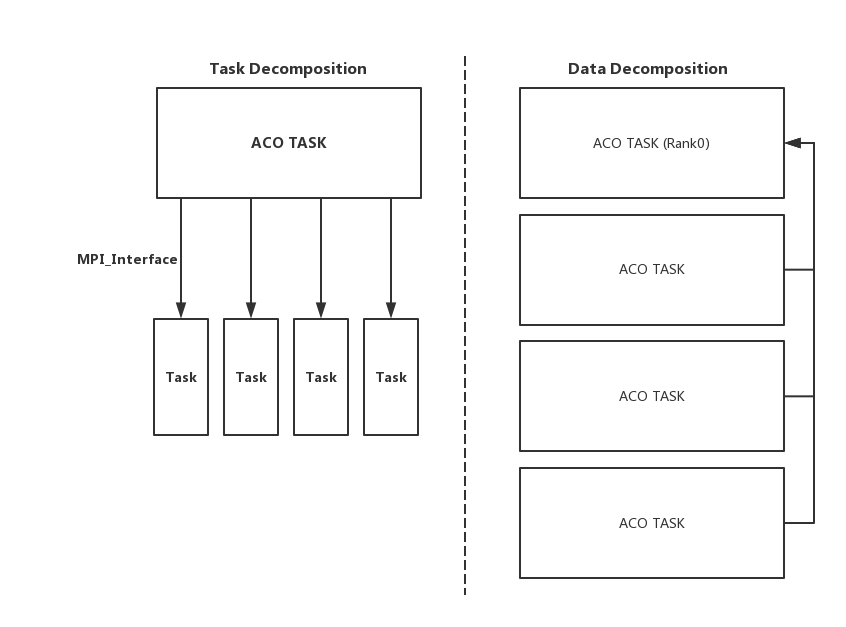
\includegraphics[width=0.7\linewidth]{parallel}
		\caption{Two types of Parallel Pattern}
		\label{fig:parallel}
	\end{figure}


	\subsection{MapReduce}
	At the beginning, I have to state that MapReduce is not the best choice for Traveling Salesman problem with Ant Colony Optimization. One of the most important concept that ACO introduced was pheromones. MapReduce does not support global variables since its data should be distributed in different data nodes. Therefore, maintain and update the pheromones data between each iteration is not feasible with MapReduce or is against the principle of this framework. \par
	There are two strategies to parallelize the ACO algorithm. First one is called chaining MapReduce jobs which contains multiple MapReduce iterations. It stores its intermediate results into binary files and read those files at the beginning of next iteration \cite{amo}. The second one takes one-iteration approach. It replicates input files and execute ACO algorithm separately and find the best result among all mappers inside the reducer. The second approach should be better than the first one according to \cite{bwu} and \cite{gc}. The processes that start the MapReduce jobs are time consuming and the number of MapReduce jobs should be as limited as possible. Therefore, we implemented the one-iteration approach with the Ant Colony Optimization algorithm. The number of mapper is determined by the number of input files. Each input file has only one line contains the coordinates of all cities. After reading the file, the first step inside each mapper is parsing the coordinates and calculate the distance between all cities. The calculation result is stored in memory so it can be accessed instantly. Then the ACO process can find the best route for this mapper. After all mapper finished their job, reducer can collect all routes and output the best one.
	\begin{figure}[H]
		\centering
		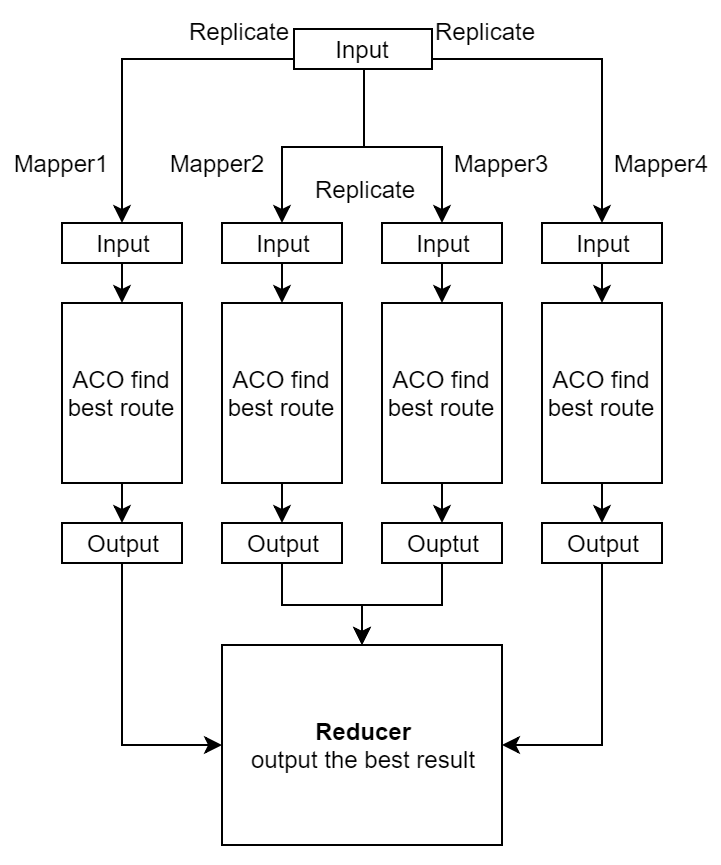
\includegraphics[width=0.4\textwidth]{mapPa}
		\caption{MapReduce single iteration}
	\end{figure}
	
	\subsection{Spark}
	In spark version of the project. We took a different approach. In the sequential version of the ant colony optimization. We instantiated a couple 2 dimensional arrays. The natural thing to do is to create a RDD for each matrix. Each of them will be updated through out the program, values in some of the matrices are dependent on other matrices. The approach we took was that we created a new Ant class that implements the Serializable class. Each Ant carries a route array that stores the route for individual ant, a ant ID number to store in ROUTES 2d array, as well as the distance of the route stored in route array. I then created a list of Ant, the size is the number of ants we want to run. I used Spark's parallelize() method to convert the list into a RDD. Now that we have a initial JavaRDD. We can start the optimization. I put all my optimization into a while loop, the loop terminals when the number of interactions we preset has been reached. In the while loop, I first broadcast my Pheromone matrix using Spark broadcast function. This is important because each iteration, the Pheromone is updated using the distance of each ant calculated from previous iteration. But in Spark, we cannot simply store the Pheromone in a global matrix and update them in the RDD. I first transform my ant RDD to a PairRDD where they key is the distance calculated, and the value is a Ant class with updated value. Inside the transformation, I let each ant calculated their own route and calculate the distance. I record the route and distance and return the Tuple. Now that I have a tuple RDD where the key is the distance, I can use RDD sortByKey function to sort the RDD. I obtain the best result from all ants by simply collect the RDD and get the first element. I use a global bestRoute variable to keep track of the best result so far. I then update the pheromone. Note that in updatePheromone function, we need the distance from all Ants to calculate delta Pheromone. We store that into a temporary array called currentLengths. The last transformation is to reset all Tuples in the RDD to original states: set each element in route array for each ant to -1, set their distance to 0, etc. 
	
	\subsection{MASS}
	MASS is agent based framework and it perfectly fits the concept of Ant Colony Optimization. Basically, ACO moves ants around the graph to find the best route, and MASS also moves Agents around the Places to process tasks. They have very similar ideas. To parallelize ACO based TSP with MASS, simply use the graph as Places, and ants as Agents. Just put all of our ACO methods into the callAll method.
	\begin{lstlisting} [format=Java, numbers=none]
	@Override
	public Object callMethod(int functionId, Object argument) {
	switch (functionId) {
	case INIT: return init();
	case CONNECT: return connectCITIES( argument);
	case SET_POSITION: return setCITYPOSITION(argument);
	case OPTIMIZE: return optimize();
	default:
	return "Unknown Method Number: " + functionId;
	}
	}
	\end{lstlisting}
	Then, for each iteration, 
	\begin{lstlisting} [format=Java, numbers=none]
	for (int i = 0; i < ITERATIONS; i++) {
	// let ants go
	ants.callAll(ACO.OPTIMIZE);
	// update pheronmen
	ants.manageAll();
	}
	\end{lstlisting}
	
	
	\section {Execution performance}
	
	\subsection{MpiJava}
	For task parallelization, computing task is split into different nodes and the exchanged data is rather small so the performance improvement is obvious. However, the Data Decomposition duplicates the whole data set to run in every node, so the performance improvement should be little.
	
	\begin{figure}[H]
		\centering
		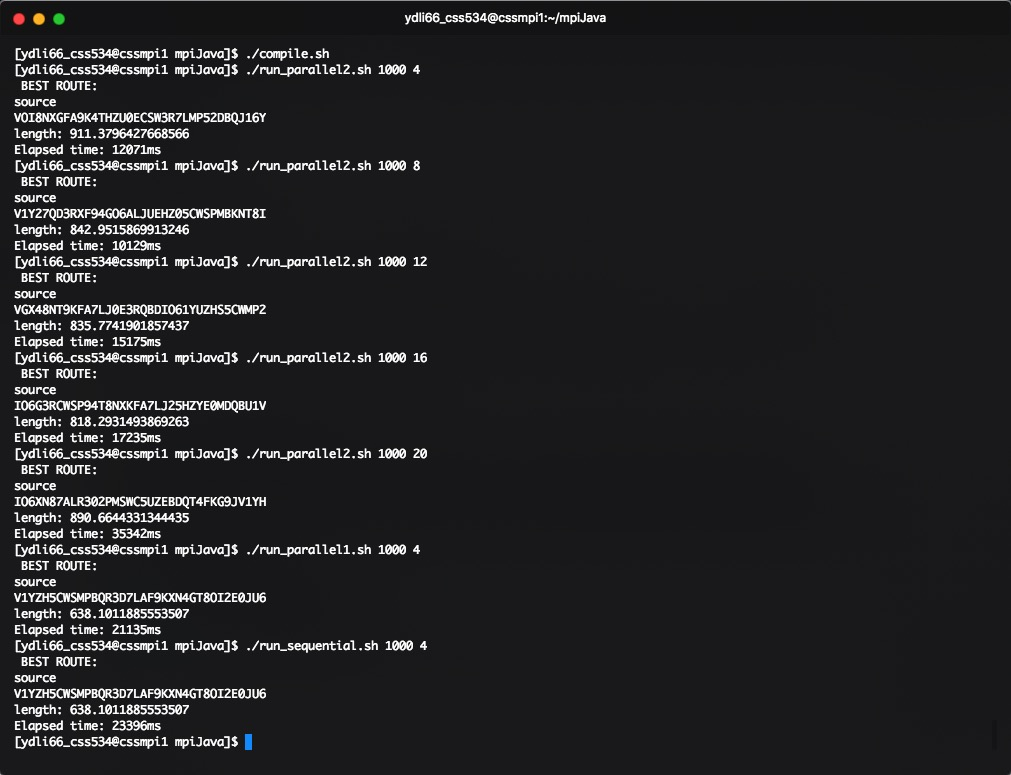
\includegraphics[width=0.7\linewidth]{running}
		\caption{Execution Snapshots}
		\label{fig:running}
	\end{figure}
	
	\subsection{MapReduce}
	The performance of MapReduce is better than we initially thought. The distance of the best route with 1000 iteration is 598. It took 44 seconds. I also tried to increase the number of iterations to 100000, and the result is 569 with 2052 seconds. However, we found the sequential version has better performance than the parallel version. This was caused by the ACO algorithm we implemented. With the similar amount of iterations, the best route it could find was almost the same. When the "mutation rate" for the ACO was increased, the results between different nodes were different, the best route was longer. To improve this, the ACO algorithm has to be adjusted with a different randomize strategy. 
	
 	\begin{figure}[H]
		\centering
		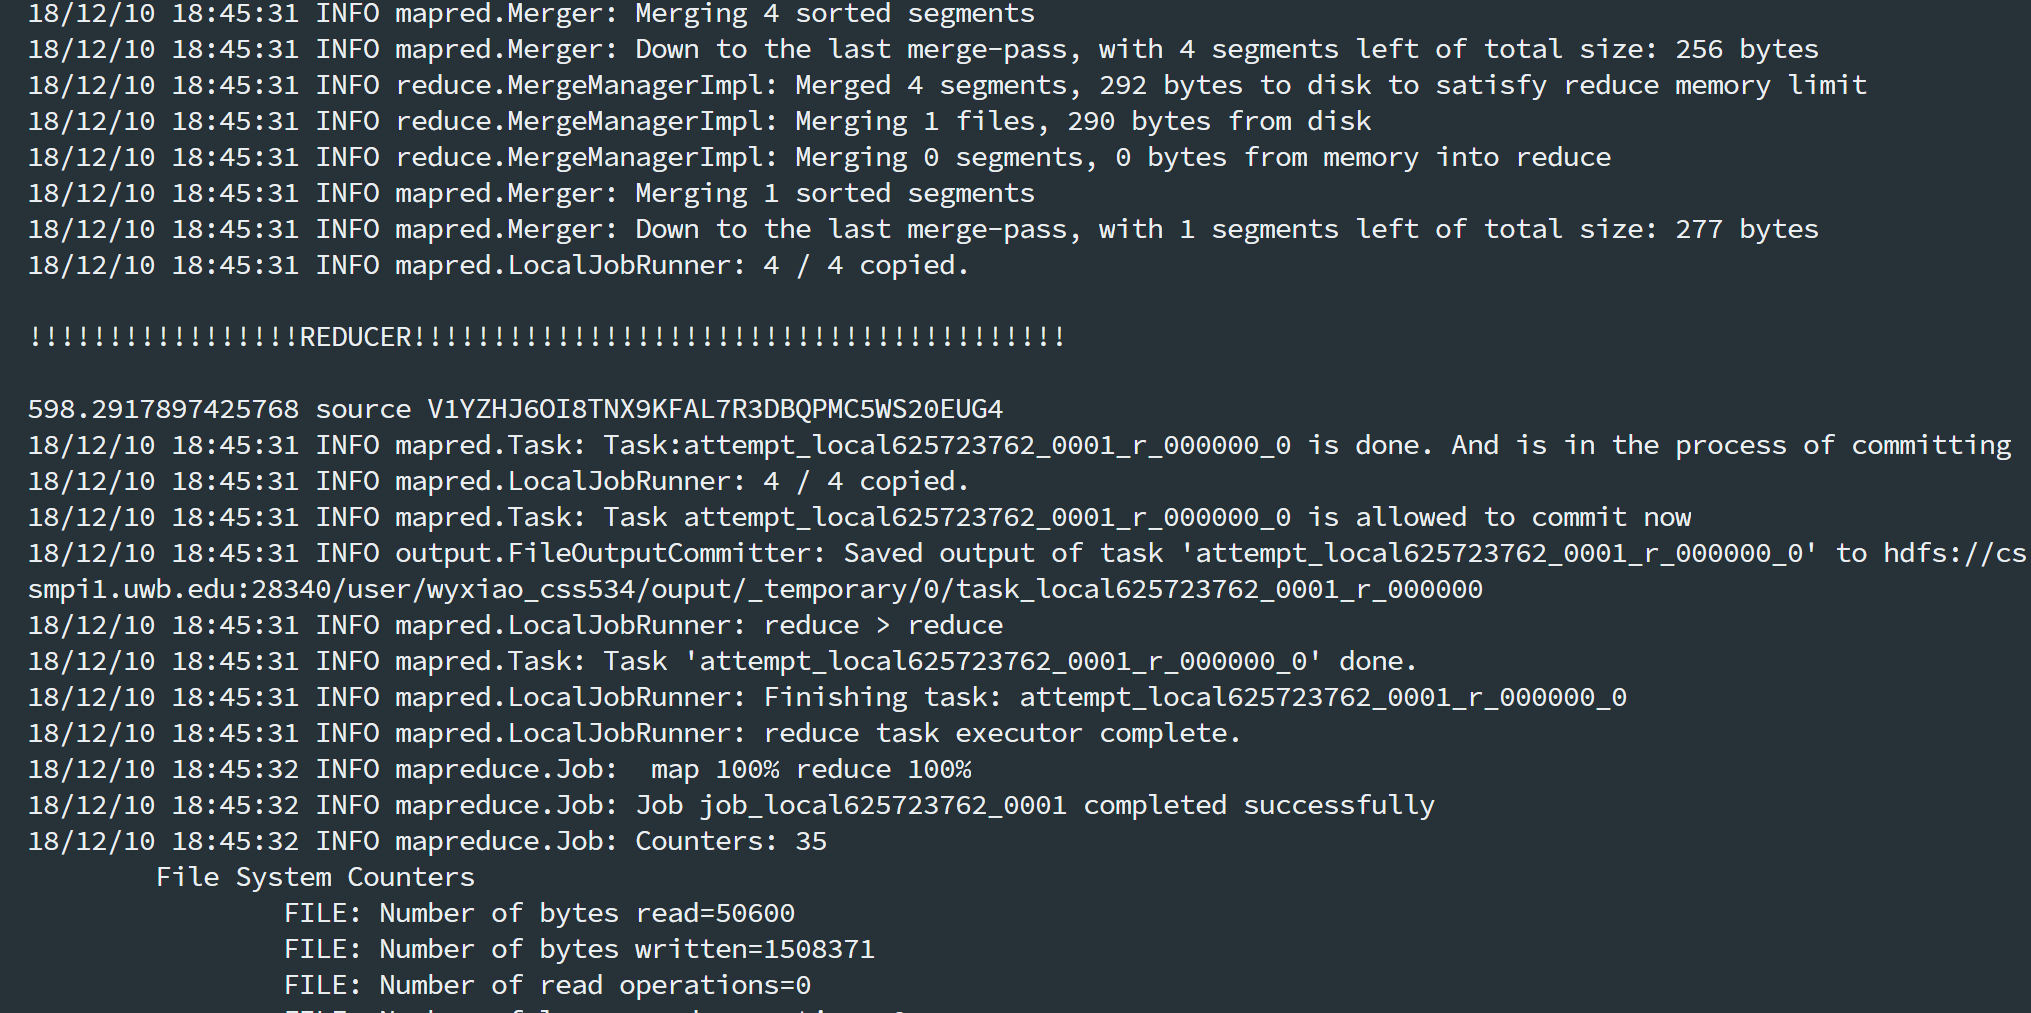
\includegraphics[width=0.7\textwidth]{mapout}
		\caption{Execution output for mapreduce}
	\end{figure}	
	
	\subsection{Spark}
	
	Unfortunately, with 1000 iterations, I only get to 1692 total distances as best route, I let the Spark program run longer and did not obtain any better results. I suspect that this is due to the fact the broadcast function may be slowing the program down by a lot. Every iteration, it needs to be recalculated to rebroadcast to all nodes. In my implementation: I let each RDD element calculate its own route, and I collect the RDD element in every iteration. there are a lot of transforming and collecting over the course of the program, it will slow down the calculation even further.
	
	\begin{figure}[H]
		\centering
		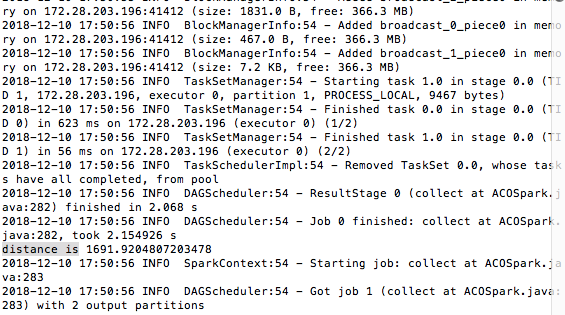
\includegraphics[width=0.7\textwidth]{sparkout}
		\caption{Execution output for spark}
	\end{figure}
	
	\subsection{MASS}
	We have finished the code for MASS, but we were not able to run it properly. We kept getting the following exception:
	\begin{lstlisting} [format=Java, numbers=none]
	Exception in thread "main" java.lang.NullPointerException
	at edu.uw.bothell.css.dsl.MASS.AgentsBase.<init>(AgentsBase.java:123)
	at edu.uw.bothell.css.dsl.MASS.Agents.<init>(Agents.java:63)
	at edu.uwb.css534.ACO_Mass.main(ACO_Mass.java:37)
	\end{lstlisting}
	This is due to the creation of \textbf{Agent} object. We have tried different parameter and passed different \textbf{Places} object, none of them worked.
	
	\subsection{Overall Performance}
	The following table compares results from each parallel technique with the same parameters and 1000 iterations
	\begin{table}[H]
		\centering
		\begin{tabular}{|c|c|c|c|c|c|}
			\hline 
			- 				& Sequential 	& MpiJava 	& MapReduce & Spark 	& MASS \\
			\hline			
			Best Length 	&738 			&  			& 598 		& 1692 		& - \\
			\hline
			Elapsed Time 	&47.468			& 	 		& 33.25		& 1140 		& - \\
			\hline
			\begin{tabular}[c]{@{}l@{}}Performance\\   Improvement\end{tabular}
							&1	 			& 			& 1.43		& 0.04		& - \\
					
			\hline
		\end{tabular}
		\caption{Performance Comparison}
	\end{table}
	
	
	
	\section {Programmability analysis}
	
	
	\subsection{MpiJava}
	
	
	\subsection{MapReduce}
	With MapRedour implementation of ACO is straightforward, every mapper runs its own ACO and report a best result at the end of all iteration. Thanks to the framework, only Mapper and Reducer class need to be implemented, the amount of boilerplate is minimal compare to other method.
	
	\subsection{Spark}
	
	Our specific implementation of the ACO may not be the best fit to be run on Spark. In general, one main advantage of Spark is the amount of boiler code can be fairly small due to the advantage of using Lamda expression. But in this program, I actually had to write more lines of code than the sequential version. The extra boilerplate code comes mainly from the work to rebroadcast Pheromone. I wrote code to broadcast it, collect distances from all ants, and then rebroadcast it after updating the Pheromone. This is because in Spark, we cannot update global data structures inside of RDD. We can read them after broadcasting it. To change a shared data structure across different nodes. I had to collect data needed to update the Pheromone in every iteration before updating it, and then rebroadcast. 
	
	\subsection{MASS}
	There is a \textbf{ACO} class in our implementation of the ACO. This class contains all ACO algorithm such as updating pheromone or move ants. To convert it to MASS, simply extend it to \textbf{Agent} and override \textit{callMethod} function. And make some adjustments to fit the MASS api. Therefore, there is only a little amount of boilerplate code and minor changes compare to our base sequential version. 
	
	\subsection{Overall Programmability}
	
	\begin{table}[H]
		\centering
		\begin{tabular}{|c|c|c|c|c|c|}
			\hline 
			- 				& Sequential 	& MpiJava 	& MapReduce & Spark 	& MASS \\
			\hline
			\begin{tabular}[c]{@{}l@{}}Proximate \\ boilerplate ratio\end{tabular}
							& 0	 			& 0.4		& 0.1		& 0.5		& 0.3 \\
			
			\hline
		\end{tabular}
		\caption{Proximate boilerplate ratio}
	\end{table}
	
	\section {Lab 5}
	
	\begin{figure}[H]
		\centering
		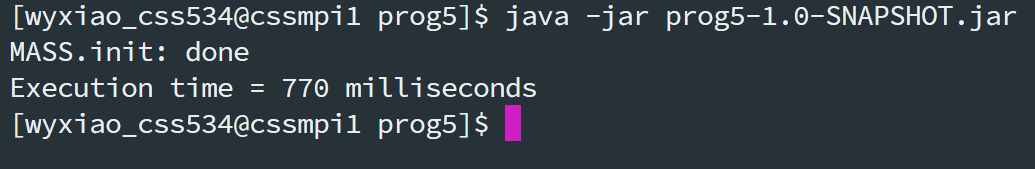
\includegraphics[width=0.7\textwidth]{lab1}
		\caption{Execution output for lab5 run sample}
	\end{figure}

	\begin{lstlisting} [format=Java]
	package edu.uwb.css534;
	
	import edu.uw.bothell.css.dsl.MASS.*; // Library for Multi-Agent Spatial Simulation
	import java.util.*;
	import java.io.*;
	import java.lang.reflect.Array;
	import java.util.Arrays;
	
	public class lab5 {
	
	private static final String NODE_FILE = "nodes.xml";
	public static void main(String[] args) throws Exception {
	MASS.setNodeFilePath(NODE_FILE);
	MASS.setLoggingLevel(LogLevel.DEBUG);
	MASS.init();
	Places matrix = new Place( 1, "Matrix", null, 10, 10);
	Agents worker = new Agents( 2, "Worker", null, matrix, 2);
	worker.callAll( Worker.goElsewhere_ );
	worker.manageAll( );
	MASS.finish();
	}
	}
	
	
	public class Worker extends Agent {
	
	public static final int goElsewhere_ = 0;
	
	public Worker() {
	super();
	}
	
	public Worker(Object object) {
	super();
	}
	
	public Object callMethod(int funcId) {
	switch (funcId) {
	case goElsewhere_:
	return goElsewhere(args);
	}
	return null;
	}
	
	public Object goElsewhere() {
	int newX = 0; // a new destination's X-coordinate
	int newY = 0; // a new destination's Y-coordinate
	int min = 1; // a new destination's # agents
	
	int currX = getPlace().getIndex()[0], currY = getPlace().getIndex()[1];
	int sizeX = getPlace().getSize()[0], sizeY = getPlace().getSize()[1];
	
	Random generator = new Random();
	boolean candidatePicked = false;
	
	int next = 0;
	next = generator.nextInt(1);
	if (next == 1) {
	newX = currX + generator.nextInt(sizeX - currX - 1);
	} else {
	newX = currX - generator.nextInt(currX);
	}
	
	next = generator.nextInt(1);
	if (next == 1) {
	newY = currY + generator.nextInt(sizeY - sizeY - 1);
	} else {
	newY = currY - generator.nextInt(currY);
	}
	
	migrate(newX, newY);
	return null;
	}
	}

	
	
	public class Matrix extends Place {
	public Matrix() { }
	public Matrix(Object obj) { }
	public Object callMethod(int method, Object o) {
	switch (method) {
	default:
	return new String("Unknown Method Number: " + method);
	}
	}
	}
	\end{lstlisting}
	
	\begin{thebibliography}{9}
		
		\bibitem{amo}
		A. Mohan and R. G, “A Parallel Implementation of Ant Colony Optimization for TSP based on MapReduce Framework,” \textit{International Journal of Computer Applications}, vol. 88, no. 8, pp. 9–12, 2014.
		
		\bibitem{bwu}
		B. Wu, G. Wu, and M. Yang, “A MapReduce based Ant Colony Optimization approach to combinatorial optimization problems,” \textit{2012 8th International Conference on Natural Computation}, 2012.
		
		\bibitem{gc}
		G. Cesari. Divi de and conquer strategies for parallel tsp heuristics.
		Comput. Oper. Res., 23:681–694, July 1996
		
	\end{thebibliography}
	
\end{document}


















